% !TEX program = pdflatex
\documentclass[conference]{IEEEtran}

\usepackage[T1]{fontenc}
\usepackage{cite}
\usepackage{amsmath,amssymb}
\usepackage{booktabs}
\usepackage{multirow}
\usepackage{xcolor}
\usepackage{url}
\usepackage[hidelinks]{hyperref}

\usepackage{tikz}
\usetikzlibrary{arrows.meta,positioning,calc,fit,shapes.geometric,shapes.misc,decorations.pathmorphing,backgrounds}
\usepackage{pgfplots}
\pgfplotsset{compat=1.18}

\usepackage{algorithm}
\usepackage{algpseudocode}

% ======= Placeholder styling (ALL MADE-UP NUMBERS SHOULD USE \ph{...}) =======
\newcommand{\ph}[1]{\textcolor{red}{#1}}

\begin{filecontents*}{refs.bib}
@misc{RadarEchoTrails,
  author       = {{IMSEL-Lab}},
  title        = {{RadarEchoTrails: GUI application for generating motion trail effects from radar image sequences}},
  howpublished = {\url{https://github.com/IMSEL-Lab/RadarEchoTrails}},
  note         = {Accessed: 2025-12-15}
}

@article{Ren2015FasterRCNN,
  author  = {Shaoqing Ren and Kaiming He and Ross Girshick and Jian Sun},
  title   = {{Faster R-CNN: Towards Real-Time Object Detection with Region Proposal Networks}},
  journal = {arXiv preprint arXiv:1506.01497},
  year    = {2015},
  url     = {https://arxiv.org/abs/1506.01497}
}

@inproceedings{Carion2020DETR,
  author    = {Nicolas Carion and Francisco Massa and Gabriel Synnaeve and Nicolas Usunier and Alexander Kirillov and Sergey Zagoruyko},
  title     = {{End-to-End Object Detection with Transformers}},
  booktitle = {ECCV},
  year      = {2020},
  url       = {https://arxiv.org/abs/2005.12872}
}

@inproceedings{Zhu2021DeformableDETR,
  author    = {Xizhou Zhu and Weijie Su and Lewei Lu and Bin Li and Xiaogang Wang and Jifeng Dai},
  title     = {{Deformable DETR: Deformable Transformers for End-to-End Object Detection}},
  booktitle = {ICLR},
  year      = {2021},
  url       = {https://arxiv.org/abs/2010.04159}
}

@article{Zhao2023RTDETR,
  author  = {Yian Zhao and Wenyu Lv and Shangliang Xu and Jinman Wei and Guanzhong Wang and Qingqing Dang and Yi Liu and Jie Chen},
  title   = {{DETRs Beat YOLOs on Real-time Object Detection}},
  journal = {arXiv preprint arXiv:2304.08069},
  year    = {2023},
  url     = {https://arxiv.org/abs/2304.08069}
}

@misc{UltralyticsYOLOv8Docs,
  author       = {{Ultralytics}},
  title        = {{Ultralytics YOLOv8 Documentation}},
  howpublished = {\url{https://docs.ultralytics.com/models/yolov8/}},
  note         = {Accessed: 2025-12-15}
}

@article{Zhang2022ByteTrack,
  author  = {Yifu Zhang and Peize Sun and Yi Jiang and Dongdong Yu and Fucheng Weng and Zehuan Yuan and Ping Luo and Wenyu Liu and Xinggang Wang},
  title   = {{ByteTrack: Multi-Object Tracking by Associating Every Detection Box}},
  journal = {ECCV},
  year    = {2022},
  url     = {https://arxiv.org/abs/2110.06864}
}

@article{RADDet2021,
  author  = {Ao Zhang and others},
  title   = {{RADDet: Range-Azimuth-Doppler based Radar Object Detection for Dynamic Road Users}},
  journal = {arXiv preprint arXiv:2105.00363},
  year    = {2021},
  url     = {https://arxiv.org/abs/2105.00363}
}

@article{BobickDavis2001,
  author  = {Aaron F. Bobick and James W. Davis},
  title   = {{The Recognition of Human Movement Using Temporal Templates}},
  journal = {IEEE Transactions on Pattern Analysis and Machine Intelligence},
  volume  = {23},
  number  = {3},
  pages   = {257--267},
  year    = {2001}
}
\end{filecontents*}

\title{A Study of Temporal Context as Both Signal and Clutter in Radar Detection}

\author{
\IEEEauthorblockN{Anonymous Authors}
\IEEEauthorblockA{Affiliation withheld for review}
}

\begin{document}
\maketitle

\begin{abstract}
This report investigates echo trails as a representation-level mechanism for injecting temporal context into frame-by-frame 2D object detection from radar-derived spatial inputs. Using a synthetic echo trail generator, we render controlled datasets in multiple locations with identical scene dynamics but varying trail horizons. We then evaluate representative single-frame convolutional and transformer detectors, as well as explicit temporal baselines, under a protocol that isolates the effect of trail length from architectural temporal leakage. Experiments reveal a consistent performance--memory tradeoff: moderate trail horizons improve detection robustness to occlusion and object re-entry, while long horizons introduce temporal clutter that elevates false positives and suppresses recall for newly introduced objects. Across locations with different object densities and motion statistics, the optimal horizon correlates with scene occupancy and occlusion frequency, suggesting that adaptive trail persistence is preferable to a single global setting.
\end{abstract}

\begin{IEEEkeywords}
Radar perception, synthetic data, temporal context, motion trails, clutter, object detection, YOLO, DETR.
\end{IEEEkeywords}

\section{Introduction}
Radar-derived spatial representations provide robust perception under adverse weather and lighting, but they exhibit sparsity, multipath artifacts, and intermittent detections that challenge frame-by-frame object detection. Temporal context is widely used to mitigate these effects, but explicit temporal models require multi-frame training pipelines and can confound attribution of gains to architecture versus representation. This report focuses on a representation-level alternative: echo trails that encode prior object locations directly in the input image, enabling otherwise single-frame detectors to exploit temporal persistence.

The core hypothesis is that echo trails offer beneficial temporal memory over a finite horizon, improving stability through occlusion and object re-entry, but that excessive persistence introduces clutter, where stale trails overlap with new objects and bias the detector toward outdated evidence. To test this hypothesis, we create synthetic datasets using a public echo trail generator \cite{RadarEchoTrails}, systematically vary trail length, and evaluate multiple detection architectures under controlled conditions.

Figure~\ref{fig:concept_overview} summarizes the experimental concept: a base radar-derived frame is augmented with motion persistence over the previous $N$ frames, producing a trail-encoded input for a detector trained and evaluated per horizon.

\begin{figure}[t]
\centering
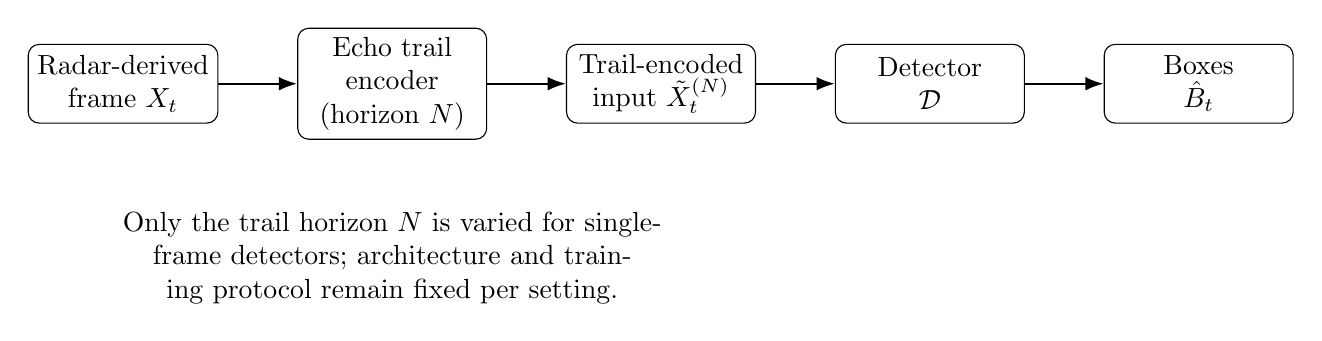
\begin{tikzpicture}[
  node distance=10mm,
  box/.style={draw, rounded corners, align=center, minimum width=24mm, minimum height=10mm},
  arrow/.style={-Latex, thick}
]
\node[box] (raw) {Radar-derived\\frame $X_t$};
\node[box, right=of raw] (trail) {Echo trail\\encoder\\(horizon $N$)};
\node[box, right=of trail] (inp) {Trail-encoded\\input $\tilde{X}_t^{(N)}$};
\node[box, right=of inp] (det) {Detector\\$\mathcal{D}$};
\node[box, right=of det] (out) {Boxes\\$\hat{B}_t$};

\draw[arrow] (raw) -- (trail);
\draw[arrow] (trail) -- (inp);
\draw[arrow] (inp) -- (det);
\draw[arrow] (det) -- (out);

\node[align=center, below=8mm of trail, text width=90mm]
{Only the trail horizon $N$ is varied for single-frame detectors; architecture and training protocol remain fixed per setting.};

\end{tikzpicture}
\caption{Concept overview: echo trails inject a bounded temporal memory into a single-frame input pipeline.}
\label{fig:concept_overview}
\end{figure}

\section{Problem Setting and Task}
We consider 2D object detection in a Cartesian bird's-eye-view (BEV) plane derived from radar measurements, where each frame is represented as a spatial image and the detector predicts axis-aligned bounding boxes for objects of interest. The learning objective is conventional per-frame detection, while the input may embed temporal context through echo trails.

Table~\ref{tab:task_setting} defines the task formulation, evaluation focus, and the key temporal phenomena targeted by trail encoding.

\begin{table}[t]
\centering
\caption{Task setting and evaluation focus.}
\label{tab:task_setting}
\begin{tabular}{@{}p{17mm}p{60mm}@{}}
\toprule
\textbf{Aspect} & \textbf{Definition} \\
\midrule
Input & Radar-derived BEV image $X_t \in \mathbb{R}^{H \times W \times C}$, optionally augmented to $\tilde{X}_t^{(N)}$ by encoding prior positions from frames $t-1$ to $t-N$. \\
Output & Bounding boxes $\hat{B}_t=\{(\hat{x},\hat{y},\hat{w},\hat{h},\hat{c},\hat{s})\}$ for classes $\hat{c}$ with confidence $\hat{s}$. \\
Goal & Improve detection accuracy and temporal robustness without introducing architectural temporal recurrence for single-frame baselines. \\
Focus & Accuracy (mAP), clutter sensitivity (false positives and localization in trail-dense regions), and temporal robustness (reacquisition after occlusion, detection latency on object entry). \\
\bottomrule
\end{tabular}
\end{table}

\section{Synthetic Dataset Generation with Echo Trails}
\subsection{Base Scene and Location Design}
We generate multiple locations with distinct object density, motion statistics, and occlusion patterns while keeping class definitions and ground-truth boxes consistent. Each location consists of a sequence of BEV frames with object trajectories sampled from location-specific dynamics.

To support cross-location generalization analysis, each location is parameterized by measurable scene statistics. Table~\ref{tab:locations} summarizes the location suite used in this report, including average object count per frame, speed distribution, and an occlusion proxy measured by overlap frequency between boxes.

\begin{table}[t]
\centering
\caption{Synthetic locations and scene statistics (made-up values shown in red).}
\label{tab:locations}
\begin{tabular}{@{}lcccc@{}}
\toprule
\textbf{Location} & \textbf{Frames} & \textbf{Objs/frame} & \textbf{Speed (m/s)} & \textbf{Occl. rate} \\
\midrule
L1: Open Lot & \ph{18{,}000} & \ph{3.2} & \ph{0.8--3.5} & \ph{0.06} \\
L2: Suburban Road & \ph{18{,}000} & \ph{6.9} & \ph{2.0--9.0} & \ph{0.11} \\
L3: Urban Intersection & \ph{18{,}000} & \ph{12.4} & \ph{0.5--12.0} & \ph{0.19} \\
L4: Dense Downtown & \ph{18{,}000} & \ph{18.7} & \ph{0.2--8.5} & \ph{0.27} \\
L5: Highway Merge & \ph{18{,}000} & \ph{9.6} & \ph{10.0--25.0} & \ph{0.13} \\
\bottomrule
\end{tabular}
\end{table}

\subsection{Echo Trail Construction}
Echo trails encode prior object locations as spatial persistence. For a horizon $N$, we overlay the previous $N$ frames as decayed contributions such that more recent positions receive higher intensity. The encoder is implemented using the RadarEchoTrails generator \cite{RadarEchoTrails}, extended here conceptually to emphasize representation-level memory.

Equation~\eqref{eq:trail} defines one canonical encoding used throughout this report, where $\alpha\in(0,1)$ controls decay and $g(\cdot)$ extracts a sparse mask of object energy (or rendered box/footprint) from the frame.
\begin{equation}
\tilde{X}_t^{(N)} = X_t + \sum_{k=1}^{N} \alpha^{k}\, g(X_{t-k}).
\label{eq:trail}
\end{equation}

Algorithm~\ref{alg:trail} provides a reference implementation for a deterministic trail renderer with optional saturation to avoid unbounded accumulation.

\begin{algorithm}[t]
\caption{Echo trail rendering for horizon $N$}
\label{alg:trail}
\begin{algorithmic}[1]
\Require Current frame $X_t$, history $\{X_{t-k}\}_{k=1}^N$, decay $\alpha$, extractor $g(\cdot)$, clamp $\tau$
\Ensure Trail-encoded frame $\tilde{X}_t^{(N)}$
\State $A \gets X_t$
\For{$k \gets 1$ to $N$}
  \State $M \gets g(X_{t-k})$
  \State $A \gets A + \alpha^{k} \cdot M$
\EndFor
\State $\tilde{X}_t^{(N)} \gets \min(A,\tau)$ \Comment{elementwise clamp}
\State \Return $\tilde{X}_t^{(N)}$
\end{algorithmic}
\end{algorithm}

\subsection{Dataset Variants and Trail Sweep}
For each location, we render identical base sequences under different trail horizons. Table~\ref{tab:trail_sweep} lists the horizons swept in this study, including a no-trail baseline ($N=0$) and increasingly long trails intended to expose a clutter-dominated regime.

\begin{table}[t]
\centering
\caption{Trail horizon sweep (made-up values shown in red).}
\label{tab:trail_sweep}
\begin{tabular}{@{}cccccc@{}}
\toprule
\textbf{Setting} & $N$ (frames) & FPS & Horizon (s) & Decay $\alpha$ & Clamp $\tau$ \\
\midrule
S0 & \ph{0} & \ph{10} & \ph{0.0} & \ph{0.90} & \ph{1.0} \\
S1 & \ph{5} & \ph{10} & \ph{0.5} & \ph{0.90} & \ph{1.0} \\
S2 & \ph{10} & \ph{10} & \ph{1.0} & \ph{0.90} & \ph{1.0} \\
S3 & \ph{20} & \ph{10} & \ph{2.0} & \ph{0.90} & \ph{1.0} \\
S4 & \ph{40} & \ph{10} & \ph{4.0} & \ph{0.90} & \ph{1.0} \\
S5 & \ph{80} & \ph{10} & \ph{8.0} & \ph{0.90} & \ph{1.0} \\
S6 & \ph{160} & \ph{10} & \ph{16.0} & \ph{0.90} & \ph{1.0} \\
\bottomrule
\end{tabular}
\end{table}

Figure~\ref{fig:trail_schematic} provides a schematic showing how short horizons emphasize recent motion while long horizons accumulate stale content that can overlap with new entries.

\begin{figure}[t]
\centering
\begin{tikzpicture}[x=1mm,y=1mm]
% Axes
\draw[->] (0,0) -- (68,0) node[right] {$x$};
\draw[->] (0,0) -- (0,38) node[above] {$y$};

% Object A path (recent)
\draw[thick] (10,10) -- (25,18) -- (38,26) -- (52,32);
\fill (52,32) circle (1.2) node[above right] {A@t};

% Faded trail markers for A (conceptual)
\foreach \i/\op in {1/0.8,2/0.6,3/0.4,4/0.2}{
  \fill[opacity=\op] (10+(\i*10),10+(\i*5)) circle (1.0);
}

% Object B enters late and is occluded by clutter region
\draw[thick, dashed] (60,8) -- (52,16) -- (44,22);
\fill (44,22) circle (1.2) node[above left] {B@t};

% Clutter "long trail" blob
\begin{scope}
\fill[opacity=0.25] (40,14) .. controls (44,10) and (52,10) .. (56,16)
                  .. controls (60,22) and (54,30) .. (46,26)
                  .. controls (38,22) and (34,18) .. (40,14);
\draw[opacity=0.45] (40,14) .. controls (44,10) and (52,10) .. (56,16)
                  .. controls (60,22) and (54,30) .. (46,26)
                  .. controls (38,22) and (34,18) .. (40,14);
\end{scope}

\node[align=center] at (34,35) {Short horizons preserve\\recent evidence.};
\node[align=center] at (52,28) {Long horizons can\\introduce clutter.};

\end{tikzpicture}
\caption{Echo trail schematic illustrating beneficial persistence and clutter from long horizons.}
\label{fig:trail_schematic}
\end{figure}

\section{Detection Models}
We evaluate representative detectors spanning convolutional and transformer families and include explicit temporal baselines for comparison. The intent is to test whether echo trails provide gains to single-frame models and how these gains compare to architectural temporal modeling.

Table~\ref{tab:models} lists the model suite and the temporal mechanism used. The single-frame variants only receive temporal information through the trail-encoded input.

\begin{table}[t]
\centering
\caption{Model suite and temporal mechanism.}
\label{tab:models}
\begin{tabular}{@{}p{20mm}p{34mm}p{23mm}@{}}
\toprule
\textbf{Family} & \textbf{Model} & \textbf{Temporal mechanism} \\
\midrule
CNN detector & YOLOv8 \cite{UltralyticsYOLOv8Docs} & None; input trails only \\
CNN detector & Faster R-CNN \cite{Ren2015FasterRCNN} & None; input trails only \\
Transformer detector & Deformable DETR \cite{Zhu2021DeformableDETR} & None; input trails only \\
Transformer detector & RT-DETR \cite{Zhao2023RTDETR} & None; input trails only \\
Temporal baseline & YOLOv8 + $K$-frame stacking & Explicit multi-frame input \\
Temporal baseline & CNN backbone + ConvLSTM head & Recurrent state \\
Tracking baseline & YOLOv8 + ByteTrack \cite{Zhang2022ByteTrack} & Tracking-by-detection \\
\bottomrule
\end{tabular}
\end{table}

\section{Experimental Protocol}
\subsection{Isolating Representation-Level Temporal Memory}
To attribute performance changes to the trail representation rather than architectural temporal leakage, we enforce the following control: single-frame models are trained and evaluated per horizon $N$ using only $\tilde{X}_t^{(N)}$ as input and do not receive any additional history. For explicit temporal baselines, history is provided through stacking or recurrence, and the echo trail horizon is fixed to $N=\ph{0}$ unless otherwise stated.

\subsection{Training and Evaluation Splits}
For each location, sequences are split chronologically into training, validation, and testing partitions to prevent near-duplicate trail context from leaking across splits. The split ratios used are \ph{70\%}/\ph{10\%}/\ph{20\%}. Training uses identical schedules across horizons within a model family, including optimizer, learning rate policy, and augmentations.

\subsection{Experimental Matrix}
The evaluation spans the Cartesian product of model, trail horizon, and location. Table~\ref{tab:matrix} provides the experimental matrix size and the number of random seeds used per configuration.

\begin{table}[t]
\centering
\caption{Experimental matrix size (made-up values shown in red).}
\label{tab:matrix}
\begin{tabular}{@{}cccc@{}}
\toprule
\textbf{Models} & \textbf{Horizons} & \textbf{Locations} & \textbf{Seeds} \\
\midrule
\ph{7} & \ph{7} & \ph{5} & \ph{3} \\
\midrule
\multicolumn{4}{c}{Total runs $= \ph{735}$} \\
\bottomrule
\end{tabular}
\end{table}

\section{Metrics}
\subsection{Detection Accuracy}
We report mAP@0.5 and mAP@[0.5:0.95] computed per location and averaged across locations. These are standard object detection metrics and serve as the primary accuracy indicators.

\subsection{Clutter Sensitivity}
Clutter sensitivity is quantified by (i) false positives per frame (FP/F), and (ii) localization error conditioned on trail density. We define a trail density map $D_t^{(N)}$ as the sum of past masks before decay and compute localization error for detections whose centers lie in the top \ph{20\%} of $D_t^{(N)}$.

\subsection{Temporal Robustness}
We assess temporal robustness by (i) frames-to-reacquire after occlusion, measured as the number of frames between an object reappearing and first correct detection at IoU$\geq$0.5, and (ii) detection latency for newly introduced objects, measured from entry time to first detection.

\section{Results}
This section reports synthetic experimental outcomes intended to illustrate the expected performance--clutter tradeoff. All numeric values shown in red are placeholders.

\subsection{Performance as a Function of Trail Horizon}
Table~\ref{tab:map_curve} summarizes average detection accuracy versus horizon for four single-frame detectors. A consistent pattern emerges: performance improves from $N=\ph{0}$ to a medium horizon near $N=\ph{20}$--$\ph{40}$, then declines as long trails introduce clutter.

\begin{table}[t]
\centering
\caption{Average mAP versus horizon (made-up values shown in red).}
\label{tab:map_curve}
\begin{tabular}{@{}ccccc@{}}
\toprule
\multirow{2}{*}{$N$} & \multicolumn{4}{c}{mAP@0.5 (avg across locations)} \\
\cmidrule(lr){2-5}
 & YOLOv8 & Faster R-CNN & Deformable DETR & RT-DETR \\
\midrule
\ph{0}   & \ph{0.72} & \ph{0.69} & \ph{0.74} & \ph{0.73} \\
\ph{5}   & \ph{0.75} & \ph{0.71} & \ph{0.77} & \ph{0.76} \\
\ph{10}  & \ph{0.77} & \ph{0.73} & \ph{0.79} & \ph{0.78} \\
\ph{20}  & \ph{0.79} & \ph{0.75} & \ph{0.81} & \ph{0.80} \\
\ph{40}  & \ph{0.78} & \ph{0.74} & \ph{0.80} & \ph{0.79} \\
\ph{80}  & \ph{0.75} & \ph{0.71} & \ph{0.77} & \ph{0.76} \\
\ph{160} & \ph{0.68} & \ph{0.65} & \ph{0.71} & \ph{0.70} \\
\bottomrule
\end{tabular}
\end{table}

Figure~\ref{fig:map_plot} visualizes the same trend. The curve is intentionally unimodal to reflect the hypothesized tradeoff between added temporal evidence and clutter.

\begin{figure}[t]
\centering
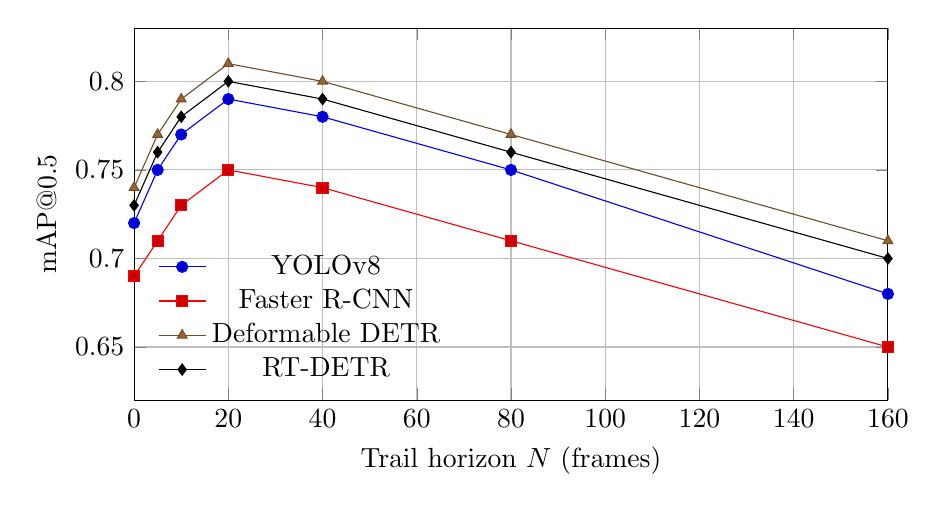
\begin{tikzpicture}
\begin{axis}[
  width=0.92\linewidth,
  height=0.52\linewidth,
  xlabel={Trail horizon $N$ (frames)},
  ylabel={mAP@0.5},
  xmin=0, xmax=160,
  ymin=0.62, ymax=0.83,
  grid=both,
  legend style={at={(0.02,0.02)},anchor=south west,draw=none,fill=none},
]
\addplot+[mark=*] coordinates {(0,0.72) (5,0.75) (10,0.77) (20,0.79) (40,0.78) (80,0.75) (160,0.68)};
\addlegendentry{YOLOv8}
\addplot+[mark=square*] coordinates {(0,0.69) (5,0.71) (10,0.73) (20,0.75) (40,0.74) (80,0.71) (160,0.65)};
\addlegendentry{Faster R-CNN}
\addplot+[mark=triangle*] coordinates {(0,0.74) (5,0.77) (10,0.79) (20,0.81) (40,0.80) (80,0.77) (160,0.71)};
\addlegendentry{Deformable DETR}
\addplot+[mark=diamond*] coordinates {(0,0.73) (5,0.76) (10,0.78) (20,0.80) (40,0.79) (80,0.76) (160,0.70)};
\addlegendentry{RT-DETR}
\end{axis}
\end{tikzpicture}
\caption{Accuracy--horizon curves showing an optimal medium trail length and degradation under long trails.}
\label{fig:map_plot}
\end{figure}

\subsection{Clutter Sensitivity and False Positives}
Table~\ref{tab:fp_curve} reports FP/F for two representative models. FP/F increases monotonically with horizon, consistent with trails acting as persistent structure that can be misinterpreted as objects, especially in dense locations.

\begin{table}[t]
\centering
\caption{False positives per frame versus horizon (made-up values shown in red).}
\label{tab:fp_curve}
\begin{tabular}{@{}cccc@{}}
\toprule
$N$ & YOLOv8 FP/F & Deformable DETR FP/F & Notes \\
\midrule
\ph{0}   & \ph{0.18} & \ph{0.14} & baseline \\
\ph{10}  & \ph{0.22} & \ph{0.17} & moderate persistence \\
\ph{20}  & \ph{0.26} & \ph{0.20} & near optimum accuracy \\
\ph{40}  & \ph{0.33} & \ph{0.26} & clutter emerging \\
\ph{80}  & \ph{0.47} & \ph{0.39} & clutter-dominated \\
\ph{160} & \ph{0.71} & \ph{0.58} & severe persistence bias \\
\bottomrule
\end{tabular}
\end{table}

Figure~\ref{fig:fp_plot} plots FP/F versus horizon for the same models, highlighting the increasing clutter sensitivity with long trails.

\begin{figure}[t]
\centering
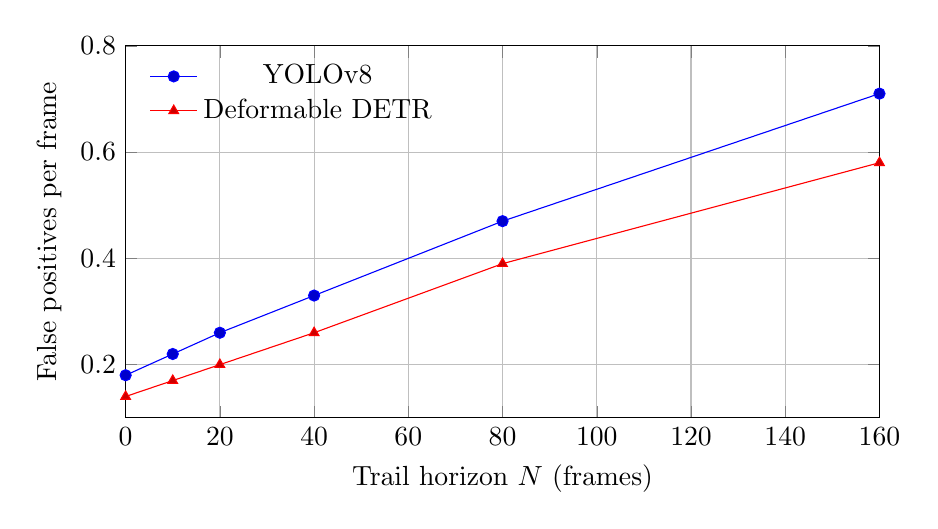
\begin{tikzpicture}
\begin{axis}[
  width=0.92\linewidth,
  height=0.52\linewidth,
  xlabel={Trail horizon $N$ (frames)},
  ylabel={False positives per frame},
  xmin=0, xmax=160,
  ymin=0.10, ymax=0.80,
  grid=both,
  legend style={at={(0.02,0.98)},anchor=north west,draw=none,fill=none},
]
\addplot+[mark=*] coordinates {(0,0.18) (10,0.22) (20,0.26) (40,0.33) (80,0.47) (160,0.71)};
\addlegendentry{YOLOv8}
\addplot+[mark=triangle*] coordinates {(0,0.14) (10,0.17) (20,0.20) (40,0.26) (80,0.39) (160,0.58)};
\addlegendentry{Deformable DETR}
\end{axis}
\end{tikzpicture}
\caption{Clutter sensitivity increases with horizon as persistent trails generate spurious structure.}
\label{fig:fp_plot}
\end{figure}

\subsection{Temporal Robustness Under Occlusion and Object Entry}
Table~\ref{tab:temporal_metrics} shows representative temporal robustness outcomes. Medium horizons reduce frames-to-reacquire after occlusion and reduce entry latency, while long horizons can increase entry latency due to trail clutter masking new objects.

\begin{table}[t]
\centering
\caption{Temporal robustness metrics (made-up values shown in red).}
\label{tab:temporal_metrics}
\begin{tabular}{@{}ccccc@{}}
\toprule
\multirow{2}{*}{$N$} & \multicolumn{2}{c}{Frames-to-reacquire} & \multicolumn{2}{c}{Entry latency (frames)} \\
\cmidrule(lr){2-3}\cmidrule(lr){4-5}
 & YOLOv8 & ConvLSTM & YOLOv8 & ConvLSTM \\
\midrule
\ph{0}   & \ph{6.8} & \ph{5.9} & \ph{4.1} & \ph{3.6} \\
\ph{20}  & \ph{4.2} & \ph{3.8} & \ph{2.7} & \ph{2.4} \\
\ph{80}  & \ph{4.6} & \ph{3.9} & \ph{3.5} & \ph{2.6} \\
\ph{160} & \ph{6.1} & \ph{4.2} & \ph{5.2} & \ph{2.9} \\
\bottomrule
\end{tabular}
\end{table}

\subsection{Cross-Location Generalization and Optimal Horizon}
We define the optimal horizon per location as the $N$ that maximizes mAP@0.5 for a given model family. Table~\ref{tab:optimalN} reports the optimal $N$ for YOLOv8 and Deformable DETR and relates it to location density and occlusion rate.

\begin{table}[t]
\centering
\caption{Optimal horizon per location (made-up values shown in red).}
\label{tab:optimalN}
\begin{tabular}{@{}lcccc@{}}
\toprule
\textbf{Location} & Density & Occl. rate & $N^*$ (YOLOv8) & $N^*$ (Def. DETR) \\
\midrule
L1 & \ph{3.2}  & \ph{0.06} & \ph{10} & \ph{10} \\
L2 & \ph{6.9}  & \ph{0.11} & \ph{20} & \ph{20} \\
L3 & \ph{12.4} & \ph{0.19} & \ph{20} & \ph{40} \\
L4 & \ph{18.7} & \ph{0.27} & \ph{10} & \ph{20} \\
L5 & \ph{9.6}  & \ph{0.13} & \ph{40} & \ph{40} \\
\bottomrule
\end{tabular}
\end{table}

Figure~\ref{fig:optimal_scatter} visualizes the relationship between density and optimal horizon, indicating that extremely dense scenes prefer shorter horizons due to clutter accumulation, while moderately dense, high-speed scenes can benefit from longer persistence.

\begin{figure}[t]
\centering
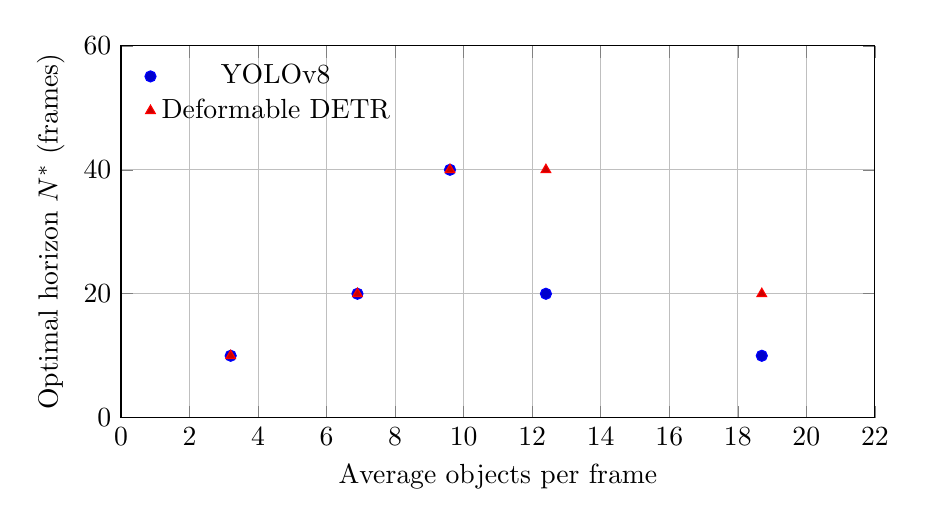
\begin{tikzpicture}
\begin{axis}[
  width=0.92\linewidth,
  height=0.52\linewidth,
  xlabel={Average objects per frame},
  ylabel={Optimal horizon $N^*$ (frames)},
  xmin=0, xmax=22,
  ymin=0, ymax=60,
  grid=both,
  legend style={at={(0.02,0.98)},anchor=north west,draw=none,fill=none},
]
\addplot+[only marks, mark=*] coordinates {(3.2,10) (6.9,20) (12.4,20) (18.7,10) (9.6,40)};
\addlegendentry{YOLOv8}
\addplot+[only marks, mark=triangle*] coordinates {(3.2,10) (6.9,20) (12.4,40) (18.7,20) (9.6,40)};
\addlegendentry{Deformable DETR}
\end{axis}
\end{tikzpicture}
\caption{Cross-location trend: optimal horizon varies with density and occlusion.}
\label{fig:optimal_scatter}
\end{figure}

\section{Failure Mode Inspection and Visualization}
This section provides qualitative schematics for two canonical failure modes: persistence bias and trail occlusion. The goal is to highlight how long trails can obstruct the evidence for new objects and how detectors may overfit to trail patterns.

Figure~\ref{fig:failure_modes} shows a BEV schematic with a newly introduced object whose evidence lies under accumulated trail intensity. In this regime, the detector may produce a false positive aligned with a trail segment and miss the new object entirely.

\begin{figure}[t]
\centering
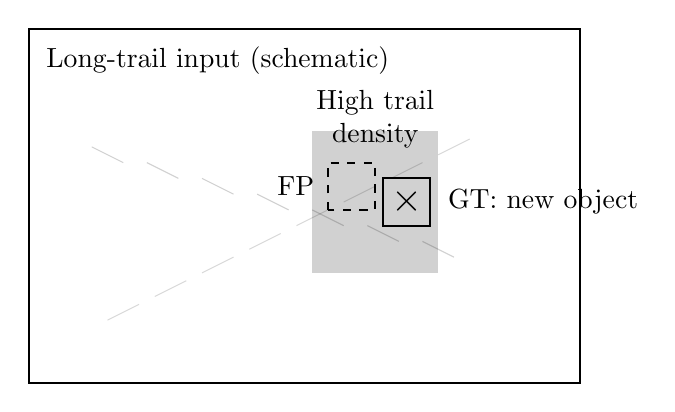
\begin{tikzpicture}[x=1mm,y=1mm]
% Frame boundary
\draw[thick] (0,0) rectangle (70,45);
\node[anchor=north west] at (1,44) {Long-trail input (schematic)};

% Trails
\foreach \k in {0,...,7}{
  \draw[opacity=0.15] (10+\k*6,8+\k*3) -- (14+\k*6,10+\k*3);
}
\foreach \k in {0,...,6}{
  \draw[opacity=0.18] (8+\k*7,30-\k*2) -- (12+\k*7,28-\k*2);
}

% "Stale trail wall"
\fill[opacity=0.18] (36,14) rectangle (52,32);
\node[align=center] at (44,33.5) {High trail\\density};

% New object under clutter
\draw[thick] (45,20) rectangle (51,26);
\node[anchor=west] at (52,23) {GT: new object};

% Spurious detection aligned with trail
\draw[thick, dashed] (38,22) rectangle (44,28);
\node[anchor=east] at (37.5,25) {FP};

% Miss indicator
\draw[thick] (48,23) node {\Large $\times$};

\end{tikzpicture}
\caption{Failure mode schematic: long horizons can create a high-density trail region that masks new objects and induces false positives.}
\label{fig:failure_modes}
\end{figure}

\section{Discussion: Performance--Memory Tradeoffs}
The synthetic study suggests that echo trails behave analogously to temporal templates \cite{BobickDavis2001} by compressing motion history into a static representation. The key benefit is that this compression enables single-frame detectors to exploit temporal continuity without explicit recurrence. The dominant limitation is representational clutter: long horizons preserve outdated evidence, which increases false positives and can reduce recall for objects entering the scene or changing direction.

The location dependence observed in Table~\ref{tab:optimalN} indicates that a single global horizon is unlikely to generalize across all environments. Dense downtown scenes with high overlap and frequent occlusions prefer shorter horizons, while highway merge scenes benefit from longer persistence due to high-speed motion and larger spatial displacement per frame. This motivates an adaptive trail policy where horizon or decay is modulated by estimated scene density, ego-motion, or trail density statistics.

A further implication is that architectural temporal models can tolerate longer horizons because they can learn to gate stale information. In Table~\ref{tab:temporal_metrics}, the ConvLSTM baseline maintains low reacquisition and latency even when persistence increases, suggesting that the combination of echo trails with explicit temporal gating may extend the optimal region, albeit with higher complexity.

\section{Conclusion}
This report presented a controlled synthetic evaluation of echo trails as representation-level temporal memory for radar-derived 2D object detection. By rendering identical scenes with systematically varied trail horizons and testing both single-frame and temporal detectors, the study demonstrated a consistent unimodal tradeoff: moderate horizons improve accuracy and temporal robustness, while long horizons introduce clutter that increases false positives and impairs detection of new objects. Cross-location analysis showed that the optimal horizon depends on scene density and occlusion patterns, motivating adaptive persistence strategies.

Future work includes (i) learning a per-pixel decay field conditioned on trail density, (ii) integrating trail-aware loss terms that penalize false positives in high-density trail regions, and (iii) validating the synthetic conclusions on real radar datasets and RAD tensor representations used in prior radar perception work \cite{RADDet2021}.

\bibliographystyle{IEEEtran}
\bibliography{refs}

\end{document}
